\documentclass[12pt]{beamer}
% \usetheme{umbc4}
\usetheme{moloch}

\usepackage{amsmath,amscd}
\usepackage{fontspec}
\usepackage{unicode-math}
\usepackage{pifont}
\usepackage{xcolor}
\usepackage[dvipsnames]{xcolor}

\definecolor{midgray}{rgb}{0.65, 0.65, 0.65}

% Set the slide body to black background with white text
\setbeamercolor{background canvas}{bg=black}
\setbeamercolor{normal text}{fg=white}

% Set the title bar to black background with white text
\setbeamercolor{frametitle}{bg=black, fg=white}

% Ensure other structural elements (bullets, etc.) are visible
\setbeamercolor{structure}{fg=white}

\setmainfont{Libertinus Serif}
\setsansfont{Libertinus Sans}
\setmathfont{STIX Two Math}

\newcommand{\FrameTitle}[2]{\frametitle{#1 \hfill \small\textnormal{\textcolor{midgray}{#2}}}}
\newcommand{\snl}{\vspace*{6pt}\\}
\newcommand{\nl}{\vspace*{1em}\\}
\newcommand{\vsp}{\vspace*{1em}}


\begin{document}
\title{\center{Module Lattice-Based \\ Post-Quantum Cryptography \snl ML-KEM and ML-DSA \\}}

\author{\center{Manipal School of Information Sciences \\ Manipal \\}}
\date{\center{Friday, 24 April 2026}}
\maketitle

\begin{frame}\FrameTitle{Lattice-Based Hard Problems}{LWE}
    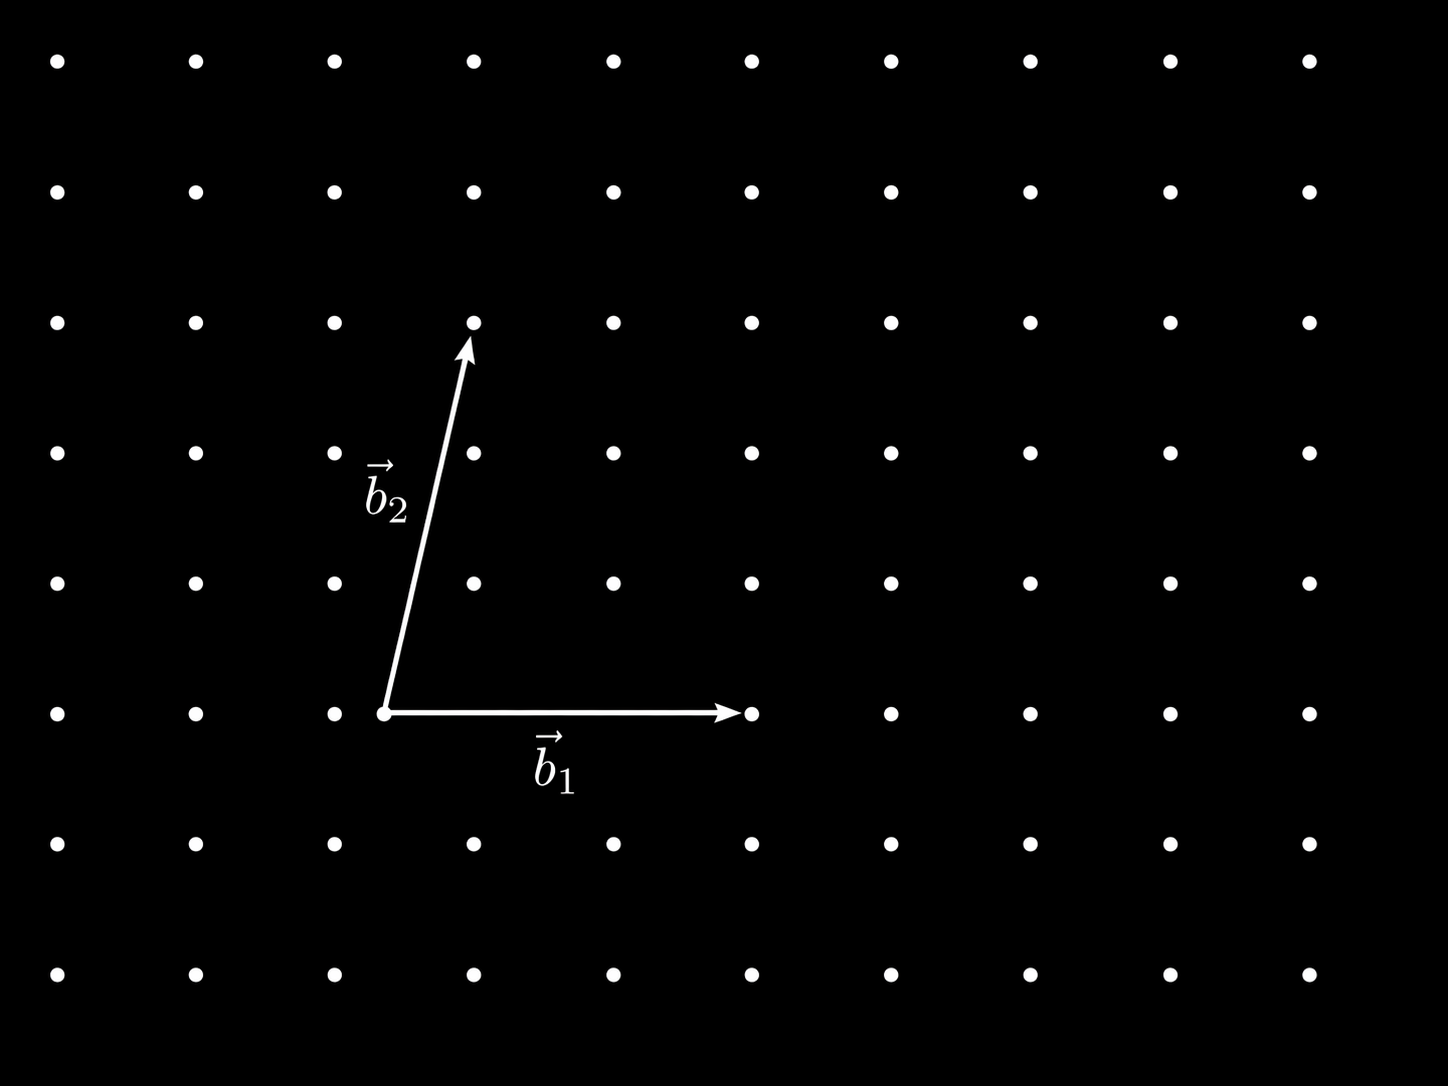
\includegraphics[width=0.9\textwidth]{images/good-basis-secret.png}
\end{frame}

\begin{frame}\FrameTitle{Lattice-Based Hard Problems}{LWE}
    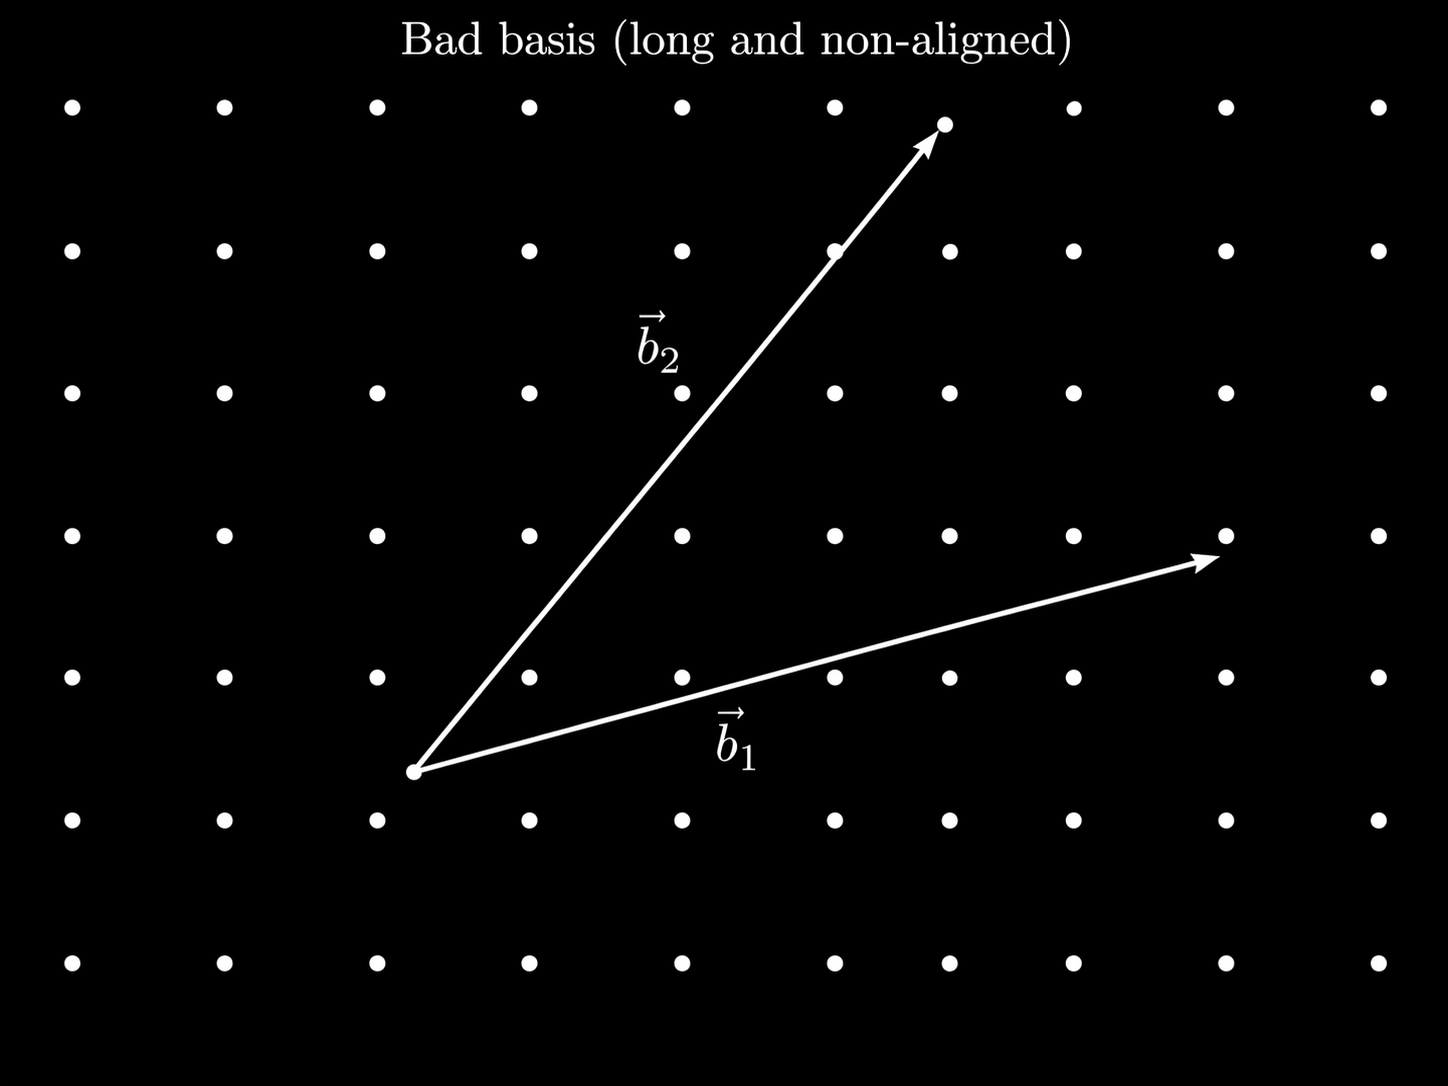
\includegraphics[width=0.9\textwidth]{images/bad-basis.png}
\end{frame}

\begin{frame}\FrameTitle{Lattice-Based Hard Problems}{LWE}
    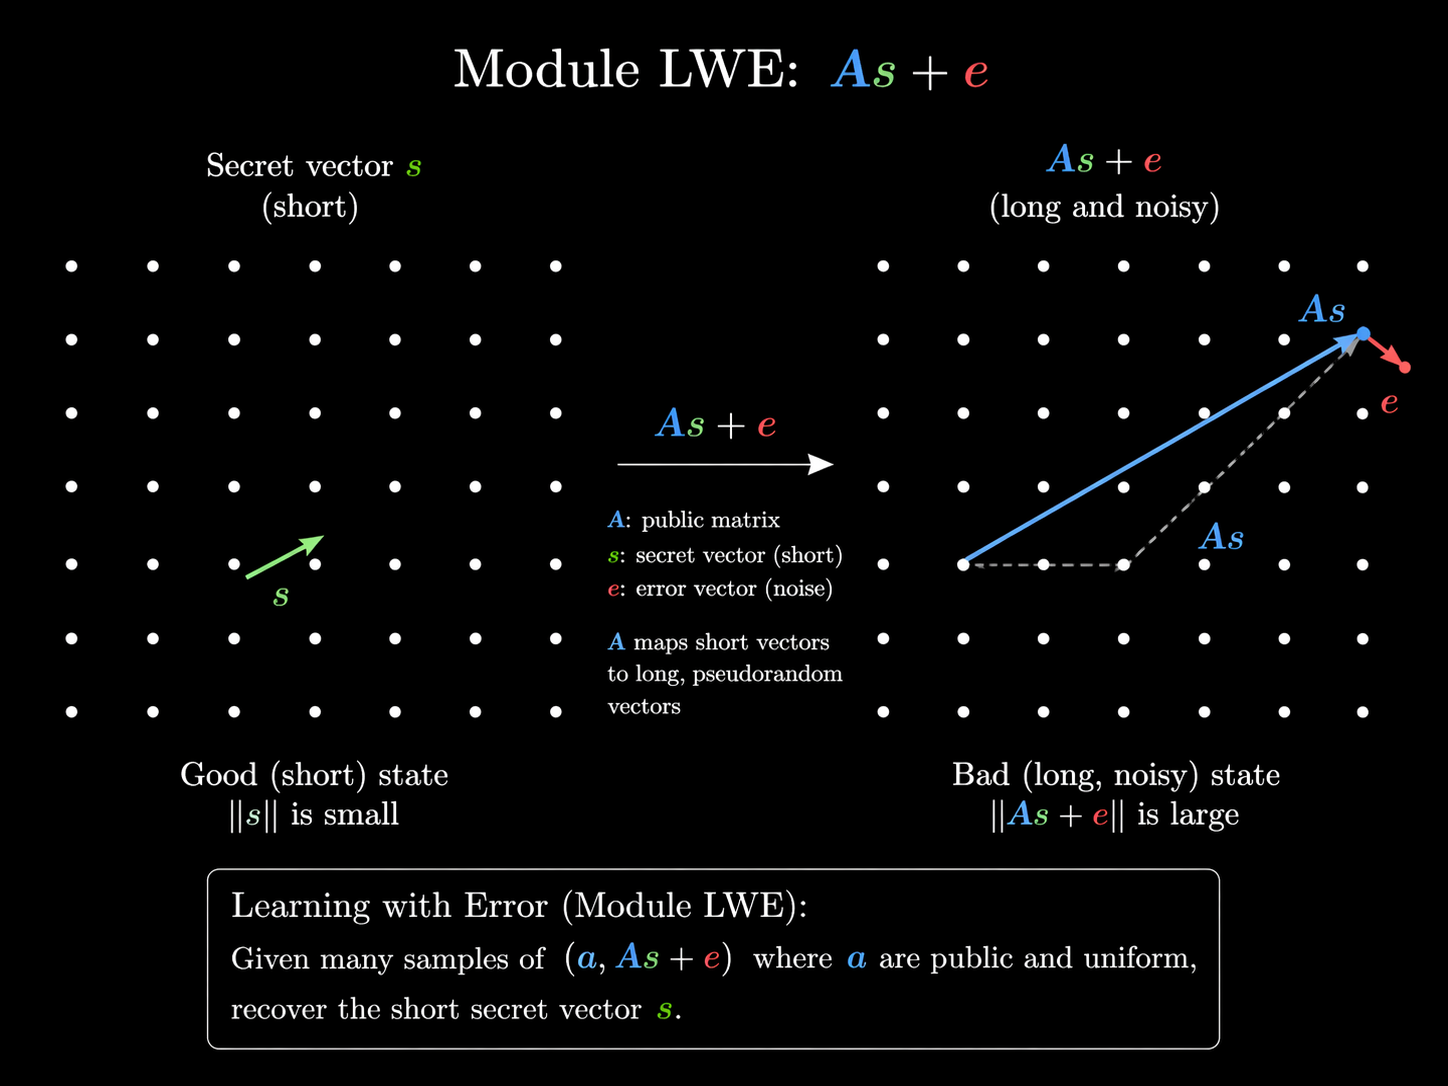
\includegraphics[width=0.9\textwidth]{images/error-vector.png}
\end{frame}

\end{document}